\documentclass[
    %draft, % Mit % kommentieren, um Bilder sichtbar zu machen und Links zu aktivieren
    pdftex,
    a4paper,
    oneside,
    parskip,
    numbers=noenddot,
    listof=totoc,
    bibliography=totoc,
    hyperfootnotes=false,
    english
]{scrreprt}
\setuptoc{toc}{totoc}

\newcommand{\thesistitle}{Identification of key information with topic analysis on large unstructured text data}
\newcommand{\thesistype}{B A C H E L O R  T H E S I S}
\newcommand{\thesistypedesc}{Department of Electrical Engineering and Computer Science \\
    University of Kassel}
\newcommand{\thesisauthorname}{Klara Maximiliane Gutekunst}
\newcommand{\thesisauthorhomestreet}{***REMOVED***}
\newcommand{\thesisauthorhometown}{34125 Kassel}
\newcommand{\thesisauthormatrikelnumber}{***REMOVED***}
\newcommand{\thesisauthoremail}{klara.gutekunst@student.uni-kassel.de}
\newcommand{\thesisdepartment}{Chair Intelligent Embedded Systems}
\newcommand{\thesisfirstreviewer}{Prof.\ Dr.\ rer.\ nat.\ Bernhard Sick}
\newcommand{\thesissecondreviewer}{Prof.\ Dr.\ Gerd Stumme}
\newcommand{\thesissupervisor}{Dr.\ Christian Gruhl}
\newcommand{\thesisdate}{\today}

% Select input encoding, usually utf8 is the best choice, on windows, \usepackage[latin1]{inputenc} maybe required
\usepackage[utf8]{inputenc}
\usepackage[T1]{fontenc}
\usepackage[english]{babel}
\usepackage{csquotes}
\usepackage{xcolor}

\MakeOuterQuote{"} % Damit ist es möglich, " " zu verwenden ohne Umlaut zu erzeugen
\defaulthyphenchar=127 % Dadurch werden auch Wörter mit Bindestrich getrennt, die schon Bindestriche enthalten.

% geometry
\usepackage[bindingoffset=1cm, left=2.5cm, right=2.5cm, top=2.5cm, bottom=2.5cm]{geometry}

% Headline
\usepackage{fancyhdr}
\pagestyle{fancy}
\renewcommand{\chaptermark}[1]{\markboth{\thechapter\ #1}{}}
\lhead{\leftmark} \rhead{\thepage}
\cfoot{}
\fancypagestyle{plain}{}

\RedeclareSectionCommand[beforeskip=1.5cm,afterskip=1cm]{chapter}

% Colors
\usepackage{color}
\usepackage{colortbl}

% Tables
\usepackage{tabularx}
\usepackage{multirow}
\setlength{\tabcolsep}{4pt}

% Drawing graphs etc.
\usepackage{pgf}
\usepackage{tikz}
\usetikzlibrary{arrows,automata}

% Footnotes
\usepackage{footmisc}
\usepackage{xspace}
\newcommand{\sic}{[\acs{sic}]\xspace}

% math
\usepackage{amsmath}
\usepackage{amssymb}

\usepackage{siunitx}

% lists
\usepackage{paralist}

% Figures
\usepackage{graphicx, wrapfig}

% Hyperlinks
\usepackage[hyphens]{url}
\usepackage{hyperref}
\hypersetup{colorlinks, citecolor=black, linkcolor=black, urlcolor=black}

% Minted
\usepackage[chapter]{minted}
%\usemintedstyle{xcode}
\setminted{frame=single,tabsize=2,linenos,autogobble}

\newmintinline[code]{text}{breaklines}

\newminted[mdcodeblock]{md}{autogobble,frame=none,linenos=false,breaklines}

% list of abbreviations
\usepackage[printonlyused]{acronym}

% Set line pitch
\usepackage{setspace}
\onehalfspacing              % anderthalbzeilig (oder auch \doublespace)

%fancyBox
%\usepackage{fancybox}

% Layout corrections (Schusterjungen)
\clubpenalty = 10000
% Layout corrections (Hurenkinder)
\widowpenalty = 10000
\displaywidowpenalty = 10000

% Figures
\usepackage{caption}
\usepackage[hypcap=true,labelformat=simple]{subcaption}
\renewcommand{\thesubfigure}{(\alph{subfigure})}
\usepackage[inkscapelatex=false]{svg}

% Tables
\usepackage{booktabs}
%\usepackage[table,xcdraw]{xcolor}

% enumerate
\usepackage{enumitem}

% Bibliography
\usepackage[square,numbers]{natbib}
\bibliographystyle{plainnat} % or plainnat abbrvnat unsrtnat

% Frequently used column types
\newcolumntype{C}[1]{>{\centering\arraybackslash}p{#1}} % centering column type with fixed width
\newcolumntype{R}[1]{>{\raggedleft\arraybackslash}p{#1}} % right aligned column type with fixed width
\newcolumntype{L}[1]{>{\raggedright\arraybackslash}p{#1}} % left aligned column type with fixed width

% Shortcuts for referencing floats:
\newcommand{\fig}[1]{\figurename~\ref{#1}} %shortcut for a figure reference
\newcommand{\tab}[1]{Table~\ref{#1}} %shortcut for a table reference
\newcommand{\eq}[1]{(\ref{#1})} %shortcut for an equation reference
\newcommand{\lst}[1]{Listing~\ref{#1}} %shortcut for a listing reference
\newcommand{\sect}[1]{Section~\ref{#1}} %shortcut for a Section reference

% Shortcut for terms
\newcommand{\databaseName}{Elasticsearch}



\begin{document}

    \pagenumbering{roman}

    \begin{titlepage}
	% Select font without serifs
	\sffamily

	% Logo
	\begin{tabularx}{\textwidth}{@{}l@{}>{\raggedleft\arraybackslash}X@{}r@{}}
		\multirow{2}{*}{
\includegraphics[width=6.8cm]{images/Logo_UniKassel}} &
		\raisebox{-1mm}{\small{Department of Electrical Engineering and Computer Science}} \\
		&\raisebox{-1mm}{\small{\thesisdepartment}} &
	\end{tabularx}

	\vspace{2.5cm}

	\begin{center}
		% Title and subtitle
		\huge{\thesistitle}

		\vspace{3cm}

		\renewcommand{\baselinestretch}{1.3}
		\Large{\thesistype}

		\large
		\thesistypedesc
	\end{center}

	\vspace{1.5cm}
	\renewcommand{\baselinestretch}{1}
	\begin{table}[htpb]
		\centering
		\begin{tabular}{ll}
			\\
			Author Name: & \thesisauthorname \\
			Address: & \thesisauthorhomestreet \\
			& \thesisauthorhometown \\
			\\
			Matriculation number: & \thesisauthormatrikelnumber \\
			E-Mail: & \thesisauthoremail \\
			\\
			Department: & \thesisdepartment \\
			\\
			Examining board 1: & \thesisfirstreviewer \\
			Examining board 2: & \thesissecondreviewer \\
			\\
			Supervisor: & \thesissupervisor \\
			\\
			Date: & \thesisdate \\
		\end{tabular}
	\end{table}

	% font with serifs
	\rmfamily
\end{titlepage}

    \chapter*{Abstract}

% Inhaltsverzeichnis und Kopfzeile
\addcontentsline{toc}{chapter}{Abstract}
% left paranthese for side header of even numbered page, right one for odd numbered page
\markboth{Abstract}{Abstract}


Finding relevant documents and connections between multiple ones becomes significantly more difficult due to the sheer amount of documents available.
Reviewing all documents in the course of the exploration of the data is no longer an option and thus, exploratory data analysis (EDA) is very important.

Institutes, such as the (German) tax offices have access to leak data containing huge amounts of documents and valuable information yet to be extracted.
However, these institutes, companies and individuals do not have sufficient resources to explore individual documents in order to find a specific one or to identify the key topics of them.
Hence, computational means, such as text mining, may facilitate the situation.
Text mining is used to automatically extract knowledge or information from unstructured text data.
Text mining is a discipline of data mining.

In this case, the starting point is a large text corpus.
Since the leaks of (German) tax offices are restricted due to confidentiality reasons, free and online accessible data for instance from Wikipedia or Twitter, containing multiple documents of unknown and diverse content will be used for this thesis.

In order to explore texts methods of topic modelling may be used.
In this thesis, these methods are first identified via literature research and applied after.
Potentially applicable methods include LDA in combination with visualisation via Wordclouds or BERTopic.


The topics to be identified can be groups of words which appear more often than the average or groups of similar documents.
Hence, a topic is not always the defined topic in terms of content, but sometimes a statistical phenomenon.
Since different methods will probably define different topics, as they work and define the meaning of 'topic' differently, their results will be compared and evaluated on the dataset.

Besides literature research, application and evaluation of the methods identified, certain preprocessing methods will probably prove to be eminent to successful work with unstructured text data.
These methods could include chunking (separating texts into equally sized segments), lemmatization (eg. faster to fast), conversion to small letters, and Part of Speech (POS) for analysis and potential exclusion of certain named entities (NER) and stop-word-lists.

First research showed that Natural Language Toolkit (NLTK) may be a library of interest in this context.

    \tableofcontents

    \chapter*{List of abbreviations}
\markboth{List of abbreviations}{List of abbreviations}

\begin{acronym}[XXXXXXXXX]
    \acro{acid}[ACID]{Atomicity, Consistency, Isolation, Durability}
    \acro{ae}[AE]{Autoencoder}
    \acro{annoy}[Annoy]{Approximate Nearest Neighbours Oh Yeah}
    \acro{api}[API]{Application Programming Interface}
    \acro{bertopic}[BERTopic]{BERT Topic Model}
    \acro{bert}[BERT]{Bidirectional Encoder Representations from Transformers}
    \acro{bilstm}[BiLSTM]{Bi-directional Long Short-Term Memory}
    \acro{bow}[BoW]{Bag of Words}
    \acro{cbow}[CBOW]{Continuous-Bag-of-Words}
    \acro{cpu}[CPU]{Central Processing Unit}
    \acro{css}[CSS]{Cascading Style Sheet}
    \acro{csv}[CSV]{Comma Separated Values}
    \acro{d2v}[Doc2Vec]{Document to Vector}
    \acro{dan}[DAN]{Deep Averaging Network}
    \acro{dbscan}[DBSCAN]{Density-Based Spatial Clustering of Applications with Noise}
    \acro{dnn}[DNN]{Deep Neural Network}
    \acro{etc}[etc.]{et cetera}    
    \acro{gb}[GB]{Gigabyte}
    \acro{glove}[GloVe]{Global Vectors}
    \acro{gpu}[GPU]{Graphics Processing Unit}
    \acro{hdbscan}[HDBSCAN]{Hierarchical DBSCAN}
    \acro{hnsw}[HNSW]{Hierarchical Navigable Small World}
    \acro{html}[HTML]{Hypertext Markup Language}
    \acro{http}[HTTP]{Hypertext Transfer Protocol}
    \acro{idf}[IDF]{Inverse Document Frequency}
    \acro{ies}[IES]{Intelligent Embedded Systems}
    \acro{ir}[IR]{Information Retrieval}
    \acro{json}[JSON]{JavaScript Object Notation}
    \acro{kl}[KL]{Karhonen-Loéve}
    \acro{knn}[kNN]{k-nearest neighbor}
    \acro{lda}[LDA]{Latent Dirichlet Allocation}
    \acro{lstm}[LSTM]{Long Short-Term Memory}
    \acro{ml}[ML]{Machine Learning}
    \acro{nli}[NLI]{Natural Language Inference}
    \acro{nlp}[NLP]{Natural Language Processing}
    \acro{nltk}[NLTK]{Natural Language Toolkit}
    \acro{nn}[NN]{Neural Network}
    \acro{nosql}[NoSQL]{Not only SQL}
    \acro{optics}[OPTICS]{Ordering Points To Identify the Clustering Structure}
    \acro{pca}[PCA]{Principal Component Analysis}
    \acro{pdf}[PDF]{Portable Document Format}
    \acro{pkl}[PKL]{Pickle}
    \acro{png}[PNG]{Portable Network Graphics}
    \acro{pvdbow}[PV-DBOW]{Distributed Bag of Words}
    \acro{pvdm}[PVDM]{Paragraph Vector Distributed Memory}
    \acro{rmse}[RMSE]{Root Mean Square Error}
    \acro{rnn}[RNN]{Recurrent Neural Network}
    \acro{rq}[RQ]{Research Question}
    \acro{rsme}[RSME]{Root Mean Square Error}
    \acro{sbert}[SBERT]{Sentence-BERT}
    \acro{snli}[SNLI]{Stanford Natural Language Inference}
    \acro{sql}[SQL]{Structured Query Language}
    \acro{ssh}[SSH]{Secure Socket Shell}
    \acro{svd}[SVD]{Singular value decomposition}
    \acro{svm}[SVM]{Support Vector Machine}
    \acro{t2v}[Top2Vec]{Topic to Vector}
    \acro{tfidf}[TF-IDF]{Term Frequency - Inverse Document Frequency}
    \acro{tf}[TF]{Term Frequency}
    \acro{ui}[UI]{User Interface}
    \acro{umap}[UMAP]{Uniform Manifold Approximation and Projection}
    \acro{url}[URL]{Uniform Resource Locator}
    \acro{use}[USE]{Universal Sentence Encoder}
    \acro{vscode}[VSCode]{Visual Studio Code}
    \acro{vsm}[VSM]{Vector Space Model}
    \acro{w2v}[Word2Vec]{Word to Vector}
    \acro{wmd}[WMD]{Word Mover's Distance}
    \acro{xml}[XML]{Extensible Markup Language}
\end{acronym}


    \pagebreak
    \pagenumbering{arabic}

    % Hier weitere Kapitel einfügen
    
Das ist die Einleitung.
"Dies ist ein Zitat"~\cite{dragon-book}.
Das ist eine Fußnote\footnote{Ich putz hier nur.}.

Abbildung~\ref{fig:uni-kassel-logo} zeigt das Logo der Uni Kassel.

\begin{figure}[htp] % htp = hier (h), top (t), oder auf einer eigenen Seite (p).
    \centering
    
\includegraphics[width=0.5\textwidth]{images/Logo_UniKassel.png} % width immer angeben!
    \caption{Das Logo der Uni Kassel}
    \label{fig:uni-kassel-logo}
\end{figure}

Listing~\ref{lst:simple-class} implementiert eine Klasse in \code{java}.

\begin{listing}[htp]
    \begin{minted}{java}
        class Foo {
            String bar;
        }
    \end{minted}
    \caption{Eine einfache Klasse}
    \label{lst:simple-class}
\end{listing}

Tabelle~\ref{tbl:evaluation-data} enthält die Daten für die Auswertung.

\begin{table}[htp]
    \centering
    \caption{Einfache Daten}
    \begin{tabular}{|l|l|l|l|}
    \hline
        Nr. & Punkte & Aufgaben & Bewertet \\
        \hline
        1  & 30 & 40 & 26 \\
        2  & 44 & 75 & 43 \\
        3  & 22 & 23 & 14 \\
        4  & 47 & 46 & 32 \\
        5  & 45 & 63 & 42 \\
        6  & 58 & 71 & 54 \\
        7  & 54 & 80 & 54 \\
        8  & 51 & 60 & 44 \\
        9  & 35 & 48 & 35 \\
        10 & 25 & 38 & 25 \\
        11 & 37 & 48 & 37 \\
        \hline
        Gesamt & 448 & 592 & 406 \\
        \hline
    \end{tabular}
    \label{tbl:evaluation-data}
\end{table}
    \chapter{Introduction}\label{ch:introduction}

\section{Motivation/ Objective}\label{sec:motivation}
Zielsetzung


\section{Related work}\label{sec:related-work}


\section{Research Questions}\label{sec:research-questions}

list of research questions
\subsection[\acs{rq}1]{\ac{rq}1: Question 1?}\label{subsec:rq1}
explanation of \ac{rq}1


\section{Structure of the Thesis}\label{sec:structure-of-the-thesis}
    \chapter{Methodology}\label{ch:methodology}

\cite{InformationRetrieval1999}

Basic concepts, methods used, etc.

\section{Preprocessing}\label{sec:preprocessing}

\subsection{Tokenization/ Chunking}\label{subsec:tokenization}

\subsection{Lemmatization}\label{subsec:lemmatization}
Type of Stemmers. Porter, Snowball, Lancaster, etc.
% https://databasecamp.de/daten/stemming-lemmatizations for difference betwee stemmers and lemmatizers
Pre-trained/defined dense vector dictionaries (Word2Vec, \ac{glove}, FastText, etc.)

\subsection{Stop-Word-Removal}\label{subsec:stop-word-removal}

\subsection{Lower case}\label{subsec:lower-case}


\section{Similarity Measurement}\label{sec:similarity-measurement}

\cite{EmbDist2015}

\subsection{Cosine Similarity}\label{subsec:cosine-similarity}

\subsection{Soft Cosine Similarity}\label{subsec:soft-cosine-similarity}

\subsection{euclidian distance}\label{subsec:euclidian-distance}

%\subsection{Hamming distance}\label{subsec:hamming-distance}

%\subsection{\ac{wmd}}\label{subsec:word-mover-distance}

%\subsection{SpaCy}\label{subsec:spacy}


\section{Embeddings}\label{sec:embeddings}

\cite{WordRep2013}
\cite{SentRep2014}

\textcolor{red}{Skizze von Pipeline für jedes Embedding, welche zeigt, wie die Daten vorverarbeitet (stemming etc.) werden/ was das Model selber macht.}

%\subsection{\ac{cbow}}\label{subsec:bag-of-words}

\subsection{\ac{d2v}}\label{subsec:doc2vec}
\cite{SentRep2014}
two flavor of doc2vec: PV-DM and PV-DBOW (https://thinkinfi.com/simple-doc2vec-explained/)
\cite{SkipGram2013}

%\subsection{\ac{w2v}}\label{subsec:word2vec}

\subsection{\ac{tfidf}}\label{subsec:tfidf}
Test test test
% svg does not icons
\begin{figure}[h] % htp = hier (h), top (t), oder auf einer eigenen Seite (p).
    \centering
    \includesvg[width=1.0\textwidth]{images/TFIDF_embedding}
    \caption{TFIDF Preprocessing}
    \label{fig:tfidf_embedding}
\end{figure}

\begin{figure}[htp] % htp = hier (h), top (t), oder auf einer eigenen Seite (p).
    \centering
    \includesvg[width=1.0\textwidth]{images/TFIDF_preprocessing}
    \caption{TFIDF Preprocessing}
    \label{fig:preprocessing}
\end{figure}

\subsection{Universal sentence encoder}\label{subsec:univ-sent-encoder}
\ac{use}
\cite{UniversalSentEnc2018}

\subsection{InferSent}\label{subsec:inferSent}
\cite{inferSent2018}

\subsection{Hugging face's sentence Transformers}\label{subsec:hf-sent-ransformers}
\cite{HfsentTrans2019}


\section{Topic Modelling}\label{sec:topic-modelling}

\subsection{\ac{bertopic}}\label{subsec:bertopic}

\subsection{\ac{lda}}\label{subsec:latent-dirichlet-allocation}

\subsection{Word Clouds}\label{subsec:word-clouds}
frequency of words in a document


\section{Appearance of documents}\label{sec:appearance}
documents saved as images in .png format, bad quality to minimize the size of the database
when querying db, top image results looked similar, which is how the idea of this section arose

\subsection{Compression of data}\label{subsec:compression}
\subsubsection{AE}\label{subsec:autoencoder}

\subsubsection{eigenface}\label{subsec:eigenface}
like pca, but for images
\cite{face-recognition2020}
\cite{face-recognition2021}
\cite{face-recognition2008}
\cite{eigenfaces2013}
\cite{eigenfaces1997}


\subsection{Clustering}\label{subsec:clustering}

Clustering is used in a variety of domains to group data into meaningful subclasses, i.e. clusters \cite{OPTICS2013, OPTICS2014, OPTICS_kMeans_2016}.
According to \citeauthor{OPTICS2013}, common domains include anomaly/ outlier detection, noise filtering, document clustering and image segmentation. 
The goal is to find clusters, which have a low inter-class similarity and a high intra-class similarity \cite{OPTICS2013}.
The similarity is measured by a distance function, which is dependent on the data type. 
Common distance functions are the Euclidean distance, the Manhattan distance and the Minkowski distance \cite{OPTICS_kMeans_2016}.

There are multiple clustering techniques, which can be divided into four categories \cite{OPTICS2016}: 
\begin{itemize}
    \item \textbf{Hierarchical clustering}:
    Algorithms, that create spherical or convex-shaped clusters, possibly naturally occurring. 
    A terminal condition has to be defined beforehand.
    Examples include CLINK, SLINK \cite{OPTICS2014} and \ac{optics} \cite{OPTICS2013}.

    \item \textbf{Partitional based clustering}: 
    Algorithms, that partition the data into $k$ clusters, whereas $k$ is given apriori.
    Clusters are shaped in a spherical manner, are similar in size and not necessarily naturally occurring.
    KMeans is a popular example of a partitional-based clustering algorithm.

    \item \textbf{Density based clustering}:
    Density is defined as the number of objects within a certain distance of each other \cite{OPTICS_kMeans_2016}.
    The resulting clusters can be of arbitrary shape and size.
    The algorithm usually chooses the optimal number of clusters given the input data.
    However, some algorithms are sensitive to input parameters, such as radius, minimum number of points and threshold.
    Popular examples are \ac{dbscan} and \ac{optics}.
    
    \item \textbf{Grid based clustering}:
    Similar to density-based clustering, but according to \citeauthor{OPTICS2016} better than density-based clustering.
    Examples include flexible grid-based clustering \cite{OPTICS2014}.
    
\end{itemize}

Multiple approaches below use the term $\varepsilon$-neighbourhood, which is defined as the set of all objects within a certain distance $\varepsilon$ of a given object \cite{OPTICS2013}.
In other words: $N_\varepsilon (x) = \left\{ y \in X | dist(x,y) \le \varepsilon, y \neq x \right\}$.


\subsubsection{KMeans}\label{subsec:kmeans}

The goal of KMeans is to partition the data into $k \in \mathbb{N}$  clusters, $k$ is given apriori \cite{OPTICS_kMeans_2016}. %
First, $k$ centroids, i.e. cluster center, are randomly initialized.
Then, the objects are assigned to the closest centroid.
Afterwards, the centroids are updated by calculating the mean of the assigned objects.
The process is repeated until the terminating condition, for instance, no more change in the clusters, is met \cite{OPTICS_kMeans_2016}.
By iteratively reassinging the objects to the closest centroid and updating the centroids, 
the algorithm minimizes the within-cluster sum of squared errors $E$, i.e. the sum of squared distances between objects in a cluster and their centroid $\mu_{i}$, 
calculated in \autoref{eq:kmeans-error} from \cite{OPTICS_kMeans_2016}, 
where $C_{i}$ is the $i$-th cluster.

\begin{equation}
    E = \sum_{i=1}^{k} \sum_{x \in C_{i}}\left\|x-\mu_{i}\right\|^{2}
\label{eq:kmeans-error}
\end{equation}

\citeauthor{OPTICS_kMeans_2016} claim, that KMeans will not identify outliers.


\subsubsection{DBSCAN}\label{subsec:dbscan}

The clusters identified by \ac{dbscan} have a high density and are separated by low-density regions \cite{OPTICS_kMeans_2016}.
In order to create clusters of minimum size and density, \ac{dbscan} distinguishes between three types of objects \cite{OPTICS_kMeans_2016}:

\begin{itemize}
    \item \textbf{Core objects}: 
    An object $x$ with at least $minPts$ objects in its $\varepsilon$-neighbourhood $N_\varepsilon(x)$.
    $N_\varepsilon(x)$ contains all objects within radius $\varepsilon$ of $x$, $\varepsilon$ being the so-called generating distance \cite{OPTICS2013}.
    In other words: The neighbourhood of $x$ has to exceed a certain threshold for $x$ to be considered a core object, i.e. $| N_\varepsilon (x) | \geq minPts$ is true.

    \item \textbf{Border objects}: 
    An object with less than $minPts$ objects in its $\varepsilon$-neighbourhood, which is in the $\varepsilon$-neighbourhood of a core object.

    \item \textbf{Noise objects}: 
    An object, which is neither a core object nor a border object.
\end{itemize}

\citeauthor{OPTICS_kMeans_2016} define $y \in X$ as directly density reachable from $x \in X$, if $y$ is in the $\varepsilon$-neighbourhood of core object $x$ \cite{OPTICS_kMeans_2016}.
Moreover, a point $y \in X$ is density reachable from $x \in X$, if there is a chain of objects $x_1, ..., x_n$ with $x_1 = x$ and $x_n = y$, 
which are directly density reachable from each other as displayed in \autoref{fig:density_reachable} \cite{OPTICS_kMeans_2016}.

\begin{figure}[htp] % htp = hier (h), top (t), oder auf einer eigenen Seite (p).
    \centering
    \includesvg[width=0.2\textwidth]{images/density_reachable}
    \caption{Density reachability cf. \cite{OPTICS1999}.
    The point $y \in X$ is density reachable from $x \in X$, since there is a chain of directly density reachable objects $x, o, y$.
    }
    \label{fig:density_reachable}
\end{figure}

The points $x \in X$ and $y \in X$ are said to be density connected, if there is an object $o$, from which both $x$ and $y$ are density reachable \cite{OPTICS_kMeans_2016}.
Density connectivity is visualized in \autoref{fig:density_connected}.

\begin{figure}[htp] % htp = hier (h), top (t), oder auf einer eigenen Seite (p).
    \centering
    \includesvg[width=0.2\textwidth]{images/density_connected}
    \caption{Density connectivity cf. \cite{OPTICS1999}.
    The objects $x$ and $y$ are density connected since there is an object $o$, from which both $x$ and $y$ are density reachable.
    }
    \label{fig:density_connected}
\end{figure}

The \ac{dbscan} algorithm starts by labeling all objects as core, border or noise points.
Then, it eliminates noise points and links all core points, which are within each other's neighbourhood \cite{OPTICS_kMeans_2016}.
Groups of connected core points form a cluster \cite{OPTICS_kMeans_2016}.
At the end every border point is assigned to a cluster \cite{OPTICS_kMeans_2016}.
The non-core point cluster assigning is non-deterministic \cite{OPTICS2013}.
This algorithm creates clusters as a maximal set of density-connected points \cite{OPTICS_kMeans_2016}.

According to \citeauthor{OPTICS_kMeans_2016}, \ac{dbscan} can identify outliers or noise.
However, the algorithm is sensitive to the input parameters $minPts$ and $\varepsilon$ and has difficulties distinguishing closely located clusters \cite{OPTICS_kMeans_2016}.
Moreover, if one wants to obtain hierarchical clustering, one has to run the algorithm multiple times with different $\varepsilon$, which is expensive in terms of memory usage \cite{OPTICS2013}.



%\subsubsection{HDBSCAN*}\label{subsec:hdbcan}


\subsubsection{OPTICS}\label{subsec:optics}

\ac{optics} does not return an explicit clustering, but rather a density-based clustering structure of the data, 
which is equivalent to clustering results of a broad range of parameters \cite{OPTICS1999}.
The idea of \citeauthor{OPTICS1999}'s approach is that real-world datasets cannot be described by a single global density, since they often consist of different local densities, 
as displayed in \autoref{fig:diff_density_cluster}.

\begin{figure}[htp] % htp = hier (h), top (t), oder auf einer eigenen Seite (p).
    \centering
    \includesvg[width=0.4\textwidth]{images/diff_density_cluster}
    \caption{Clusters of different densities cf. \cite{OPTICS1999}.
    Since $C_1$ and $C_2$ have different densities than $A$ and $B$, a clustering algorithm using one global density parameter would detect the clusters $A$, $B$ and $C$, 
    rather than $A$, $B$, $C_1$ and $C_2$ .
    }
    \label{fig:diff_density_cluster}
\end{figure}

Opposed to \ac{dbscan}, \ac{optics} is able to detect clusters of varying densities \cite{OPTICS2014}.
\ac{optics} produces an order of the elements according to the distance to the already added elements \cite{OPTICS2014, OPTICS2013}:
The first element added to the order list is arbitrary.
$\varepsilon$ defines the neighbourhood radius, i.e. the maximum distance between two elements, which are still considered to be in the same neighbourhood \cite{OPTICS_kMeans_2016}.
The order list is iteratively expanded by adding the element of the $\varepsilon$-neighbourhood to the order list, which has the smallest distance to any of the elements already in the order list.
Hence, clusters with higher density, i.e. lower $\varepsilon$, are added first (prioritized) \cite{OPTICS_kMeans_2016, OPTICS1999}.
When there are no more elements in the $\varepsilon$-neighbourhood to add, the process is repeated for the other clusters.
The non-core point cluster assigning is non-deterministic \cite{OPTICS2013}.

\begin{equation}
    RD(y) = \left\{
    \begin{array}{ll}
    \textrm{NULL} & \, \textrm{if |}N_\varepsilon (x)| < minPts \\
    max(core\_dist(x), dist(x,y)) & \, \textrm{otherwise} \\
    \end{array}
    \right. 
    \label{eq:optics-reachability-distance}
\end{equation}

\ac{optics} saves the reachability distance $RD(y)$, as calculated in \autoref{eq:optics-reachability-distance} from \cite{OPTICS2013},
with core distance core\_dist being the minimal distance $\varepsilon^{min}$ such that $| N_{\varepsilon^{min}} (x) | \geq minPts$ 
(the distance to the $minPts^{th}$ point in $N_\varepsilon$) or NULL else, 
of each element to its predecessor in the order list and thus, 
a representation of the density necessary to keep two consecutive objects in the same cluster \cite{OPTICS2013}.
If $\varepsilon < RD(y)$, then $y$ is not density reachable from any of its predecessors and thus, 
one can determine whether two points are in the same cluster for given information saved by \ac{optics} \cite{OPTICS2013, OPTICS1999}.
If the core distance of an element is not NULL, i.e. it is a core object, and it is not density reachable from its predecessors, it is the start of a new cluster \cite{OPTICS1999}.
Otherwise, the element is a noise point \cite{OPTICS1999}.
According to \citeauthor{OPTICS2013}, the algorithm builds a spanning tree, which enables obtaining the clusters for a given $\varepsilon$ by returning the connected components 
of the spanning tree after omitting all edges with $\varepsilon < RD(y)$ \cite{OPTICS2013}.
The relationship between $\varepsilon$, cluster density and nested density-based clusters is displayed in \autoref{fig:nested_density_cluster}.

% nested clusters, eps, fixed minPts
\begin{figure}[htp] % htp = hier (h), top (t), oder auf einer eigenen Seite (p).
    \centering
    \includesvg[width=0.5\textwidth]{images/nested_density_cluster.svg}
    \caption{The relationship between $\varepsilon$, cluster density and nested density-based clusters cf. \cite{OPTICS1999}.
    For a constant $minPts$, clusters with higher density such as $C_1$, $C_2$ and $C_3$, i.e. a low $\varepsilon_2$ value, 
    are completely contained in lower density clusters such as $C$ given $\varepsilon_1 > \varepsilon_2$.
    This idea forms the basis of \ac{optics} of expanding clusters iteratively and thus, 
    enables the detection of clusters for a broad range of neighbourhood radii $0 \le \varepsilon_i \le \varepsilon$.
    }
    \label{fig:nested_density_cluster}
\end{figure}

Hence, this procedure enables the extraction of clusters for arbitrary $0 \le \varepsilon_i \le \varepsilon$ \cite{OPTICS_kMeans_2016, OPTICS1999}.
According to \citeauthor{OPTICS2013}'s work, even though the clustering algorithm is expensive the extraction only needs linear time.
According to \cite{OPTICS1999}, the algorithm yields good results if the input parameters $minPts$ and $\varepsilon$ are "large enough" and thus, the algorithm is rather insensitive to the input parameters.

% effect of eps (reachability plot)
The smaller $\varepsilon$ is chosen, the more objects will be identified as noise and thus, the algorithm will not identify clusters with low density, 
since some objects only become core objects for a larger $\varepsilon$ \cite{OPTICS1999}.
According to \citeauthor{OPTICS1999}, the optimal value for $\varepsilon$ creates one cluster for most of the objects with respect to a constant $minPts$,
since information about all density-based clusters for $\varepsilon_i < \varepsilon$ is preserved.
A heuristic for choosing $\varepsilon$ based on the expected $k$-nearest neighbour distance is presented in \cite{OPTICS1999}.

% effect of minPts (reachability plot)
High values for $minPts$ smoothen the reachability curve, even though the overall shape stays roughly the same \cite{OPTICS1999}.
According to \citeauthor{OPTICS1999}, the optimal value for $minPts$ is between 10 and 20.

% TODO: reachability plot for doc images  (32x32 greyscale images and euclidean distance as similarity measure)
Similar to the approach from \cite{OPTICS1999}, \ac{optics} was used to cluster the images of the first page of documents in this work.
The images were preprocessed to 32x32 greyscale pixels as visualized in \autoref{fig:preprocessed_docs}.
The reachability distance ordered by \ac{optics} is displayed in \autoref{fig:reachability_plot}.
The resulting clusters are displayed in \autoref{fig:optics_cluster}.
Example instances of both clusters (cluster and noise) are displayed in \autoref{fig:example-cluster}.

\begin{figure}[htp] % htp = hier (h), top (t), oder auf einer eigenen Seite (p).
    \centering
    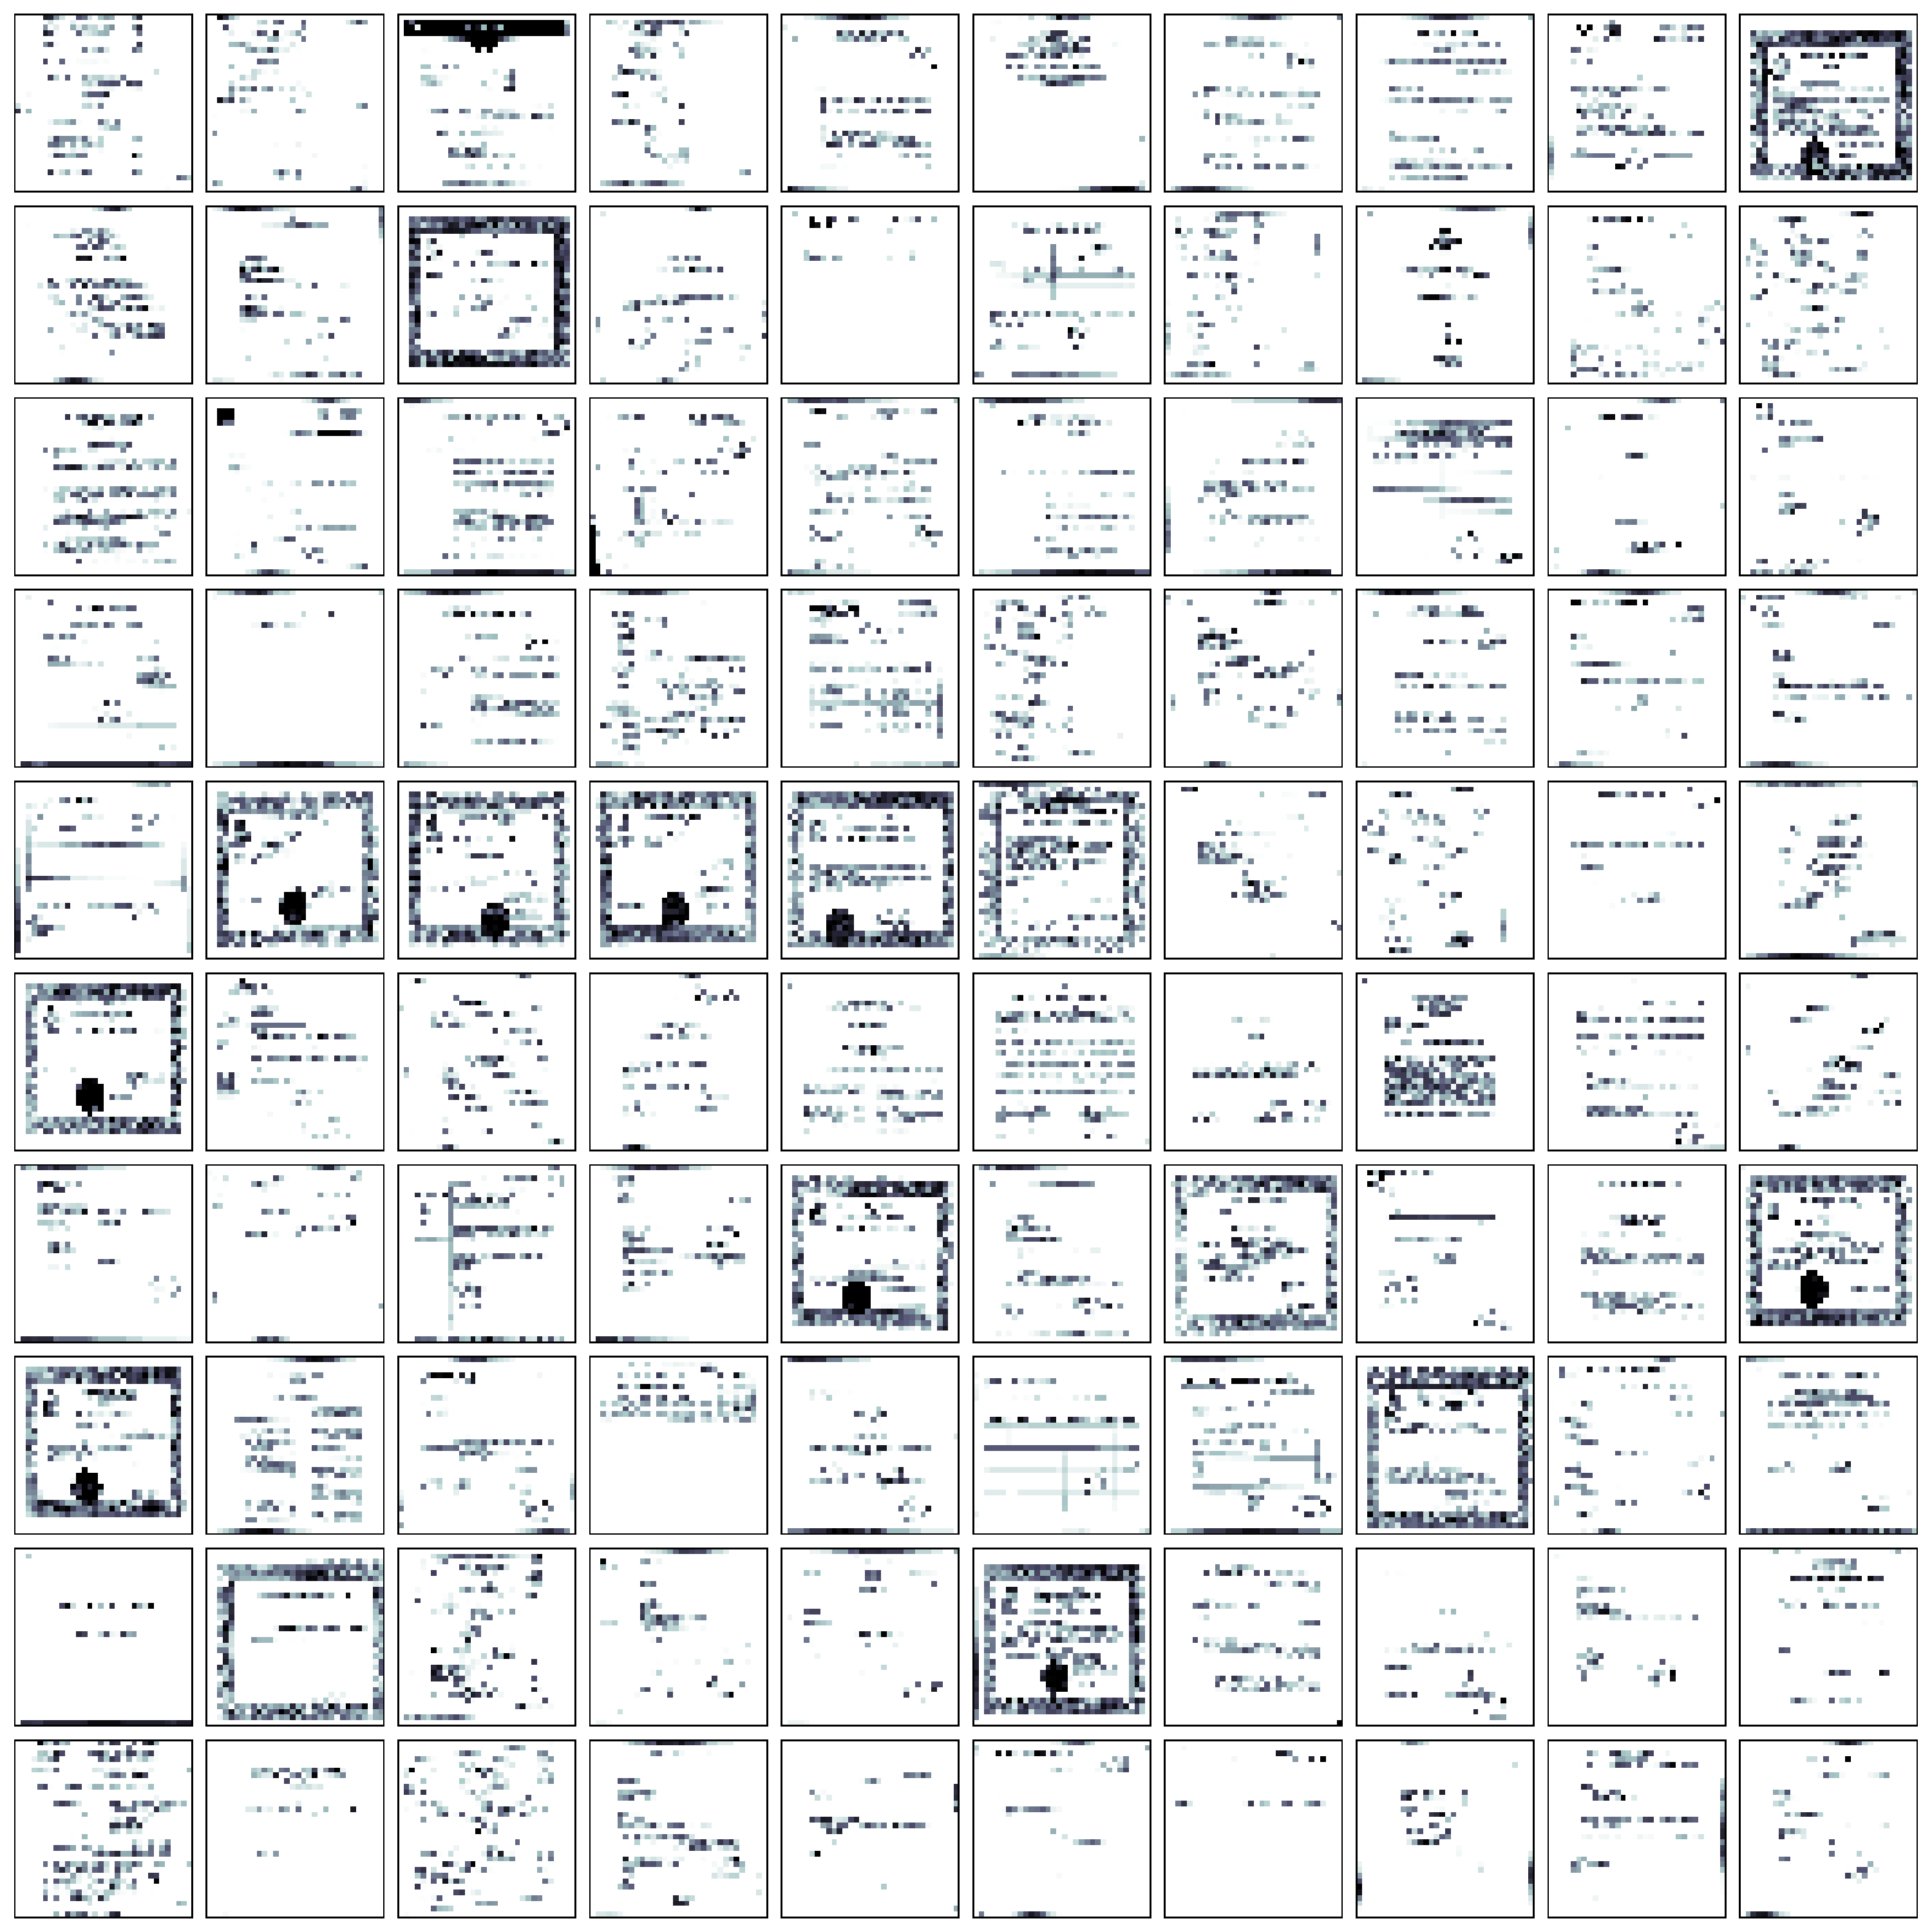
\includegraphics[width=0.5\textwidth]{images/preprocessed_docs.pdf}
    \caption{The first 100 preprocessed documents of the dataset.
    They were preprocessed in order to have the same characteristics as the images used in \cite{OPTICS1999}.
    The images were preprocessed to 32x32 greyscale pixels, which drastically reduced the quality of the images.
    }
    \label{fig:preprocessed_docs}
\end{figure}


\begin{figure}[htp] % htp = hier (h), top (t), oder auf einer eigenen Seite (p).
    \centering
    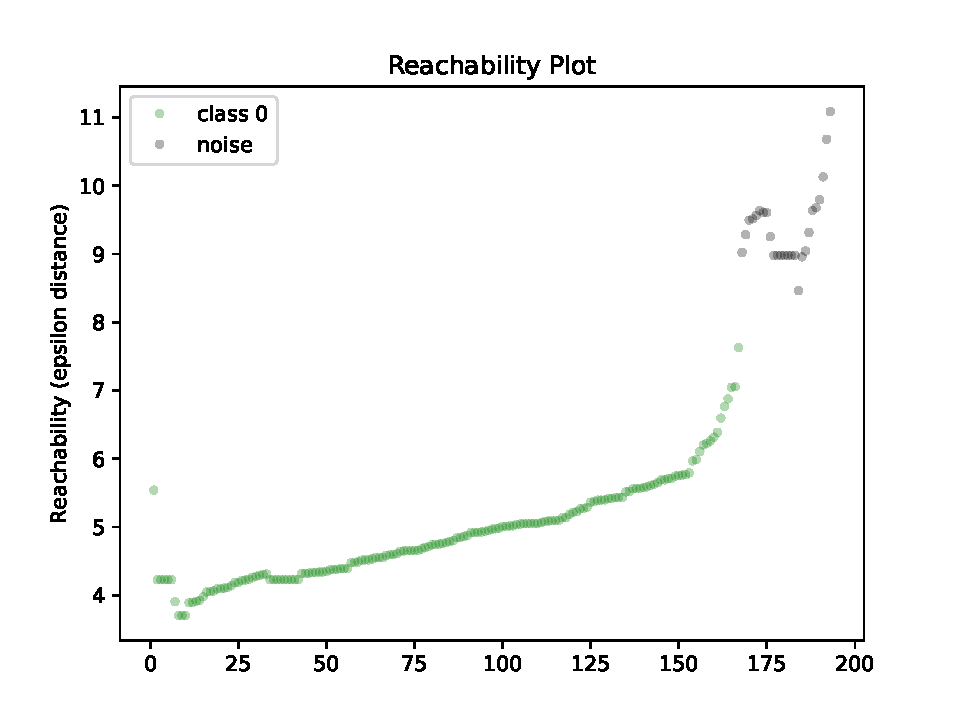
\includegraphics[width=0.5\textwidth]{images/reachability_plot.pdf}
    \caption{The reachability plot of the preprocessed documents.
    The plot was created using the \ac{optics} algorithm from the Python library scikit-learn.
    The plot shows the reachability distance of each document to its predecessor in the order list.
    The reachability distance is the minimum distance necessary to keep two consecutive objects in the same cluster.
    The plot shows that the documents are divided into a cluster and a noise region.
    }
    \label{fig:reachability_plot}
\end{figure}


\begin{figure}[htp] % htp = hier (h), top (t), oder auf einer eigenen Seite (p).
    \centering
    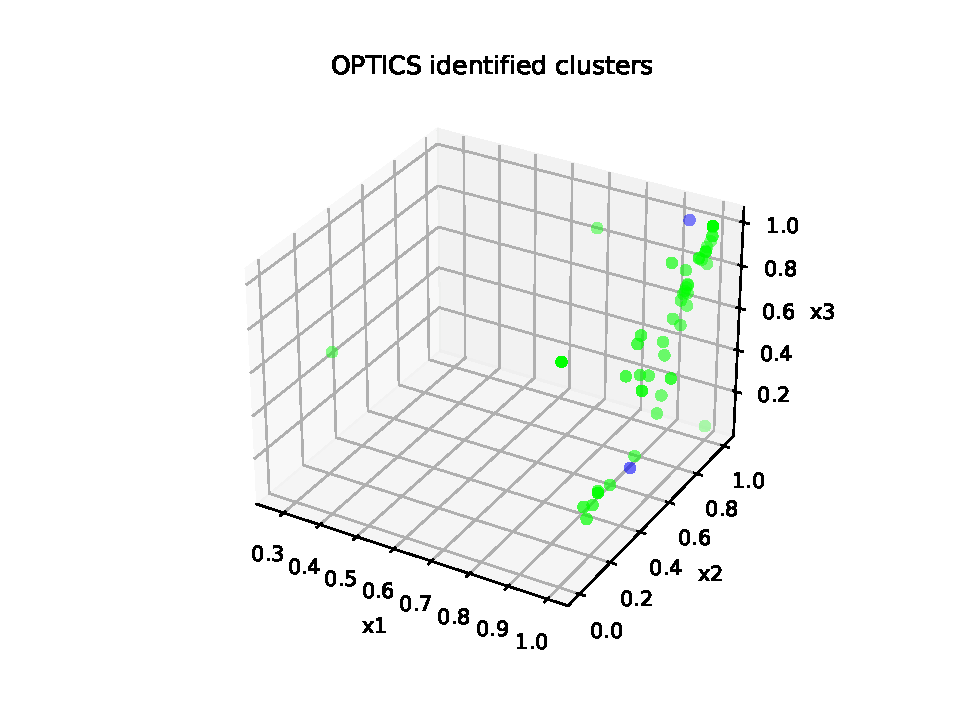
\includegraphics[width=0.5\textwidth]{images/OPTICS_cluster.pdf}
    \caption{The clusters of the preprocessed documents in a three-dimensional space.
    The clusters were extracted from the reachability plot in \autoref{fig:reachability_plot}.
    The green points belong to the cluster, whereas the blue points are noise points.
    }
    \label{fig:optics_cluster}
\end{figure}

\begin{figure}%
    \centering
    \subfloat[\centering Example image from cluster 0. The image seems to be a normal, non-certificate document.]{{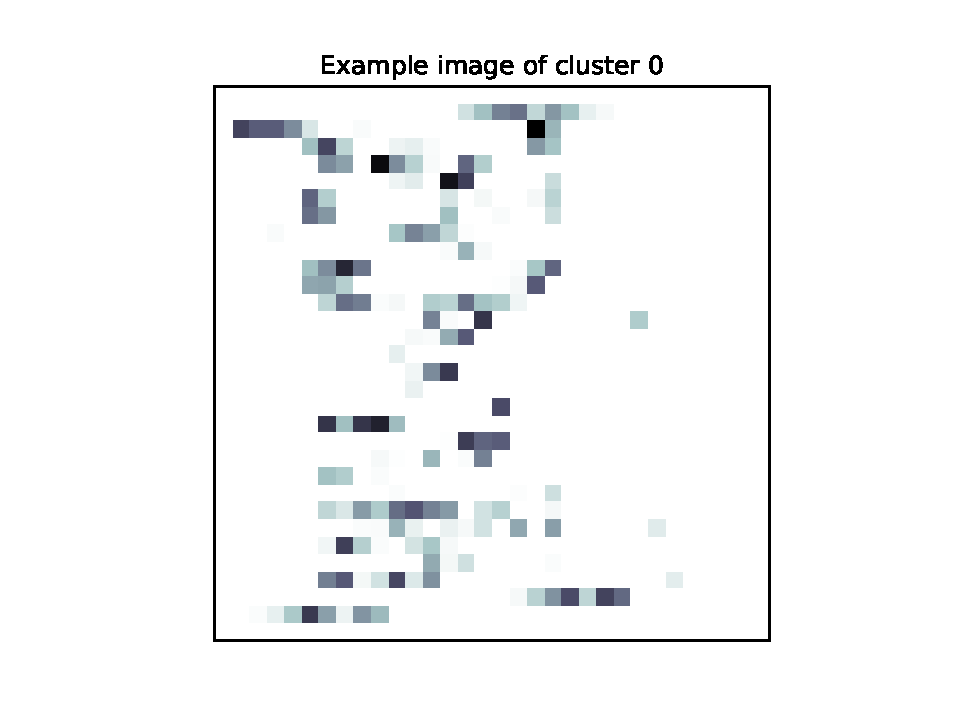
\includegraphics[width=5cm]{images/example_image_cluster_0.pdf} }}%
    \qquad
    \subfloat[\centering Example image which was identified as noise. The image seems to be a certificate.]{{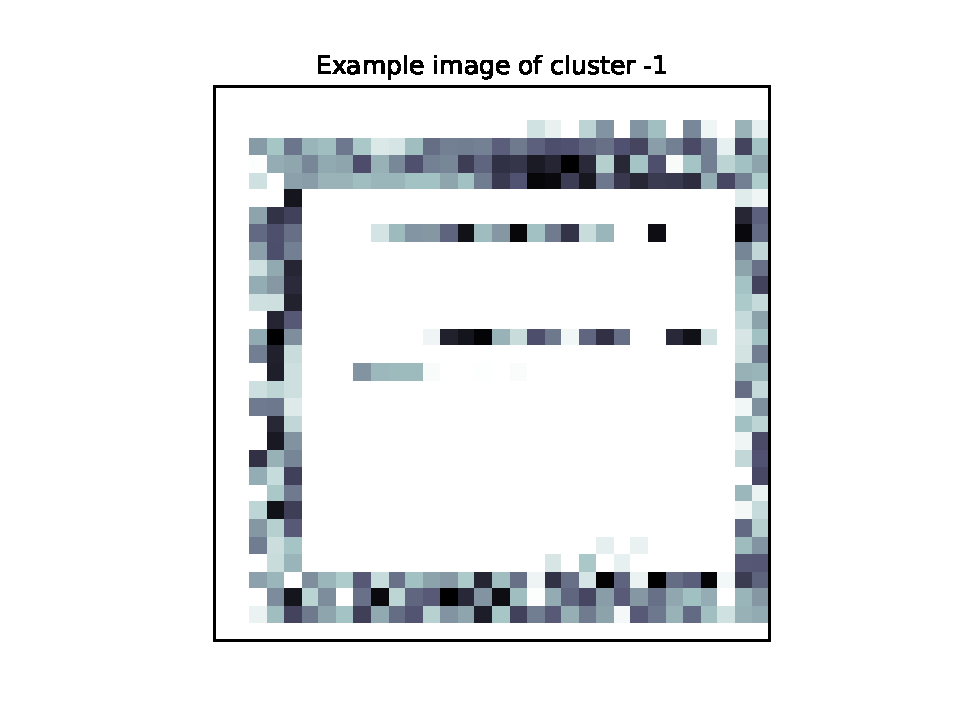
\includegraphics[width=5cm]{images/example_image_cluster_-1.pdf} }}%
    \caption{When using \ac{optics} with the configurations stated above, only one cluster and noise was identified.
    This result could be due to the degradation of quality in the context of preprocessing the images.}%
    \label{fig:example-cluster}%
\end{figure}
    \newcommand{\databaseName}{Elasticsearch}
\chapter{Implementation}\label{ch:implementation}


\section{Slurm}\label{subsec:slurm}
\cite{slurm2003}
\cite{slurm-online}




\section{Database Elasticsearch}\label{subsec:db}
% introduction, users
\databaseName{} is a widely used non-relational database, which was designed to store and perform full-text search on large corpus of unstructured data \cite{Elasticsearch2017}.
This open-source distributed document-driven database system is build in Java and is based on the Apache Lucene (Java) library for high-speed full-text search \cite{Elasticsearch2017,Elasticsearch2019}.
According to \cite{Elasticsearch2019}, \databaseName{} provides Wikipedia's full-text search and suggestions as well as Github's code search and Stack Overflow's geolocation queries and related questions.
Needless to say, \databaseName{} is prone to handle Big Data and enables near real-time search by index refreshing periods of one second.

% structure
\databaseName{}'s entries, i.e. documents are stored in logical units, so called indices.
% index
As stated in \citeauthor{Elasticsearch2019} and \citeauthor{Elasticsearch2017}'s work, the indices are structured similar to Apache Lucene's inverted index format.
An index can be spread into multiple nodes.
A node is single running instance of \databaseName{} \cite{Elasticsearch2019}.
An index is divided into one or more shards, which can be stored on different servers and enable parallelization \cite{Elasticsearch2019}.

% document
\databaseName{} indices' entries are documents, which are saved in a \ac{json} fromat \cite{Elasticsearch2017}.
A document's fields and field types are defined by the user when initializing the database index.
By default, every field of a document is indexed and searchable \cite{Elasticsearch2019}.

% Replicas
Replicas are copies of shards, which create redundancy and thus, ensure availability \cite{Elasticsearch2019}.

% content
The database is filled once with data from a large unstructured corpus of \acp{pdf}.
After the initialization of the database, it is used for queries. 
Therefore, the procedure is carries out in a completely offline fashion.

The index \textit{Bahamas} stores different embeddings of the text layer information and metadata of the documents.
As depicted in \autoref{fig:pdf2db}, not only textual information is stored in the database, but also the images of the first page of the \acp{pdf}.
The structure of the index is presented in \autoref{tbl:Elasticsearch-fields}.

% Please add the following required packages to your document preamble:
% \usepackage[table,xcdraw]{xcolor}
% If you use beamer only pass "xcolor=table" option, i.e. \documentclass[xcolor=table]{beamer}
\begin{table}[]
    \caption{Fields in \databaseName{} database in index \textit{Bahamas}}
    \begin{tabular}{|
    >{\columncolor[HTML]{EFEFEF}}l |p{0.63\textwidth}|}
    \hline
    \cellcolor[HTML]{C0C0C0}\textbf{field name} & \cellcolor[HTML]{C0C0C0}\textbf{field description}                                       \\ \hline
    \_id                                        & unique identifier of document \texttt{i}                                                 \\ \hline
    doc2vec                                     & doc2vec embedding of \texttt{i}                                                          \\ \hline
    sim\_docs\_tfidf                            & sim\_docs\_tfidf embedding + all-zero flag of \texttt{i}                                 \\ \hline
    google\_univ\_sent\_encoding                & google\_univ\_sent\_encoding embedding of \texttt{i}                                     \\ \hline
    huggingface\_sent\_transformer              & huggingface\_sent\_transformer embedding of \texttt{i}                                   \\ \hline
    inferSent\_AE                               & inferSent\_AE embedding of \texttt{i}                                                    \\ \hline
    pca\_image                                  & two dimensional \ac{pca} version of first page image of \texttt{i}                      \\ \hline
    pca\_kmeans\_cluster                        & Cluster of \texttt{i} identified by KMeans on \ac{pca} version of image                 \\ \hline
    text                                        & text of \texttt{i}                                                                       \\ \hline
    path                                        & path on local maschine to \texttt{i}                                                     \\ \hline
    image                                       & image of first page of \texttt{i}                                                        \\ \hline
    \end{tabular}
    \label{tbl:Elasticsearch-fields}
\end{table}

\begin{figure}[htp] % htp = hier (h), top (t), oder auf einer eigenen Seite (p).
    \centering
    \includesvg[width=0.7\textwidth]{images/PDFs_to_database}
    \caption{\acp{pdf} to Database. 
    The first page of the \acp{pdf} are converted to images and the complete text is extracted. 
    The images are stored in the database as well as the text and different embeddings of the text.
    }
    \label{fig:pdf2db}
\end{figure}

% query (endpoints)
% get: search id
By specifying the unique \texttt{\_id} of a document and the database \texttt{index}, it is possible to retrieve a specific document from the database using the \texttt{GET \ac{api}}.
The query is real-time by default.
The parameter \texttt{\_source\_excludes} or \texttt{\_source\_includes} may be used to exclude or include specific fields of the document in the response \cite{Elasticsearch-get}.

% full-text search
The keyword used when performing full-text search in this case is \texttt{match}.
To query for a specific value, one has to specify the \texttt{<field>} of interest and the query value.

\databaseName{} preprocesses the query value before starting the search \cite{Elasticsearch-text-analyser}.
The default preprocessing steps of the so-called default analyser include tokenization and lowercasing \cite{Elasticsearch-standard-analyser}. 
Omitting stop words is disabled by default, but it is possible to provide custom stop words or use the English stop word list \cite{Elasticsearch-standard-analyser}.
It is possible to create custom tokenizers, which split the query value into tokens of a certain maximum length.
In this work, the default analyser is used for the full-text search, since for instance configuring a maximum token length did not seem necessary or likely to improve the results.

Another useful feature of \databaseName{} is the multi-terms synonym expansion.
When the user queries a specific phrase \databaseName{} expands the query to include synonyms of the query terms \cite{Elasticsearch-synonyms}.
The maximum number of expansion terms is set to 50 by default, but can be configured by the user \cite{Elasticsearch-match}.
By default, the multi-terms synonym expansion option is enabled \cite{Elasticsearch-match}.

\databaseName{} also provides the option to perform fuzzy matching instead of exact search.
By enabling the fuzzy matching option, a \databaseName{} query consisting of for instance, \textit{Bahama} returns documents which have the word \textit{Bahamas}.
By default this option is not enabled, but can be enabled and configured individually by the user \cite{Elasticsearch-match}.
In this work, the fuzzy matching option is set to \texttt{AUTO}, which means in terms of keyword or text fields that the allowed Levenshtein Edit Distance, 
i.e. number of characters changed to create an exact match between two terms, to be considered a match, is correlated to the length of the term \cite{Elasticsearch-fuzziness}.
By default, terms of length up to two characters must match exactly, terms of length three to five characters must have an edit distance of one and 
terms of length six or more characters must have an edit distance of two \cite{Elasticsearch-fuzziness}.

% knn-search
Another search option of \databaseName{} is the \ac{knn} search.
The return value of a \ac{knn} search are the \texttt{k} nearest neighbors in terms of a certain distance function of a query vector \cite{Elasticsearch-kNN-HNSW}.
According to \citeauthor{Elasticsearch-kNN-HNSW}, one of \ac{knn} search's use cases is semantic document retrieval, which makes it a good fit for this task.
The query is a dense vector of the same dimension as the (dense) vectors stored in the database.
According to \cite{Elasticsearch-knn}, the \ac{knn} either returns the exact brute-force nearest neighbors or approximate nearest neighbors calculated by the \textcolor{red}{TODO:}\ac{hnsw} algorithm \cite{Elasticsearch-kNN-HNSW, Elasticsearch-knn}.
In this work, the approximate nearest neighbors search is used, since it is faster and the results are good enough for the use case of this work.
\ac{hnsw} is a graph-based algorithm \cite{Elasticsearch-kNN-HNSW}.
The term \texttt{navigable} refers to the graphs used, which are graphs with (poly-)logarithmic scaling of links traversed during greedy traversal with respect to the network size \cite{Elasticsearch-kNN-HNSW}.
The idea of a \texttt{hiercharical} algorithm is to create a multilayer graph, grouping links according to their link length, as displayed in \autoref{fig:hnsw-layer}. 
The search starts on the uppermost layer, i.e. the layer containing the longest links, greedily traversing the layer until reaching the local minimum.
It uses this local minimum as the starting point at the next lower layer and the process is repeated until the lowest layer is reached \cite{Elasticsearch-kNN-HNSW}.
The layers of the graph are built incrementally, and a neighbour selection heuristic, as depicted in \autoref{fig:hnsw-heuristic}, not only creates links between close elements, 
but also between isolated clusters to ensure global connectivity \cite{Elasticsearch-kNN-HNSW}.

\begin{figure}[htp] % htp = hier (h), top (t), oder auf einer eigenen Seite (p).
    \centering
    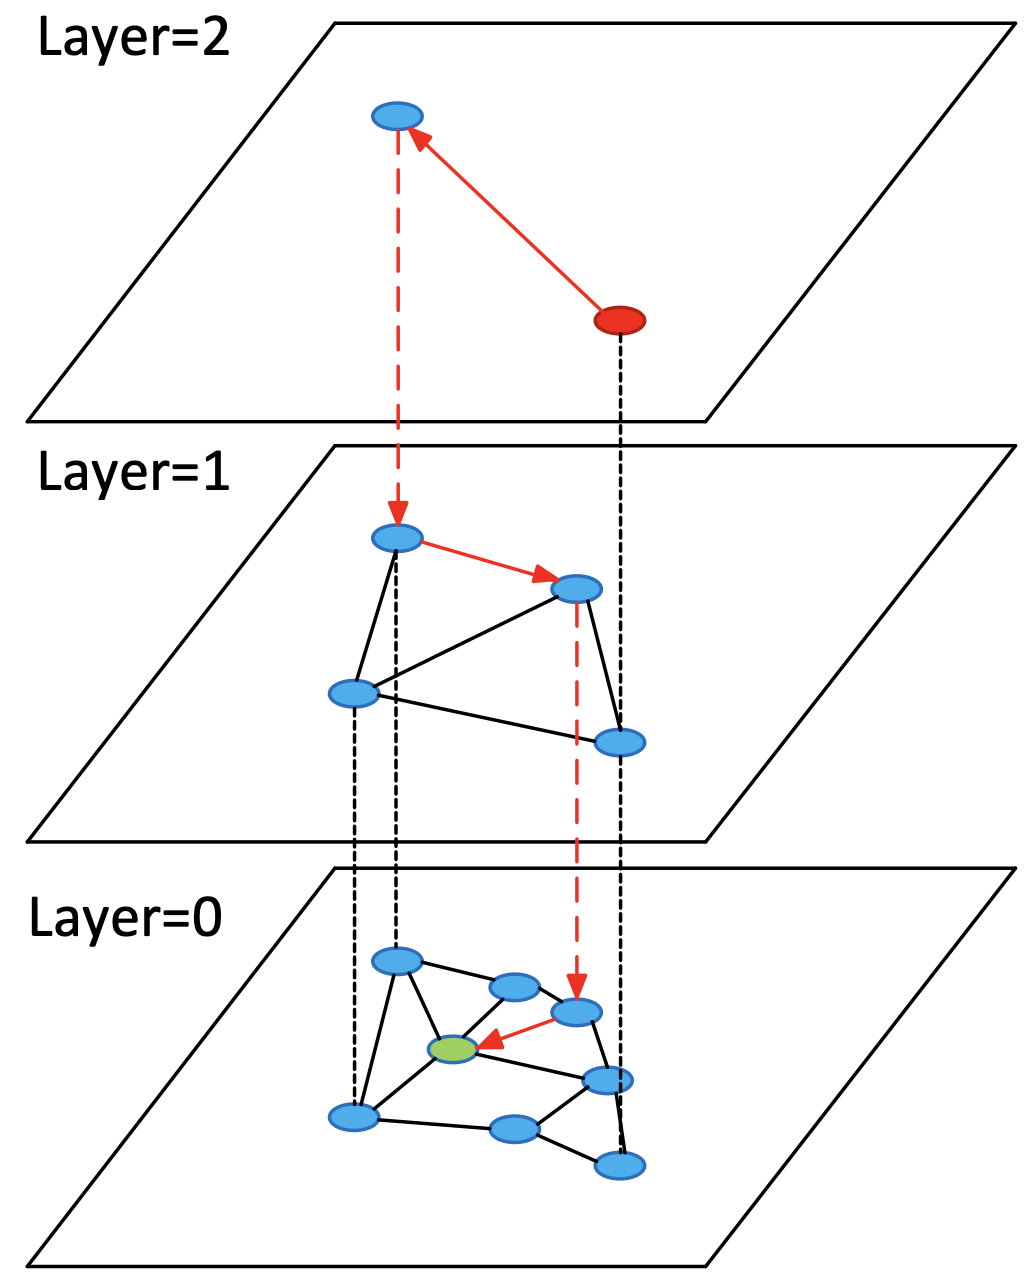
\includegraphics[width=0.4\textwidth]{images/HNSW-layer.png}
    \caption{Structure of \ac{hnsw} layer from \cite{Elasticsearch-kNN-HNSW}.
    The search starts on the uppermost layer, i.e. the layer containing the longest links, greedily traversing the layer until reaching the local minimum.
    The local minimum is used as the starting point at the next lower layer and the process is repeated until the lowest layer is reached.
    }
    \label{fig:hnsw-layer}
\end{figure}

\begin{figure}[htp] % htp = hier (h), top (t), oder auf einer eigenen Seite (p).
    \centering
    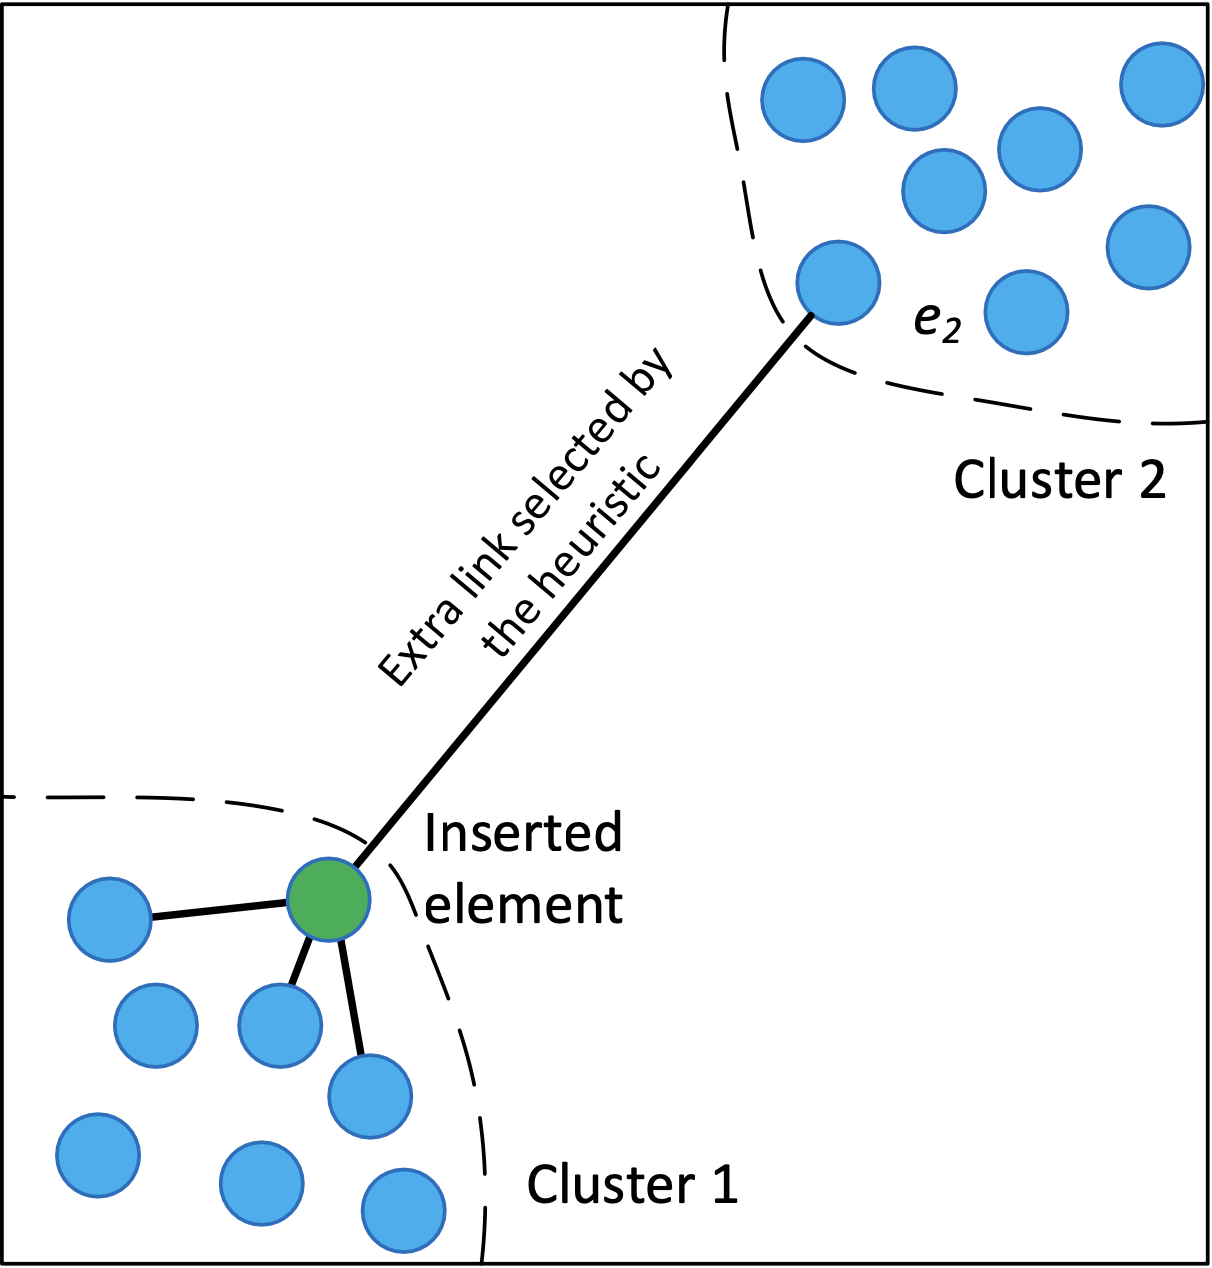
\includegraphics[width=0.4\textwidth]{images/HNSW-neighbour-selection-heuristic.png}
    \caption{Neighbour selection heuristic of \ac{hnsw} from \cite{Elasticsearch-kNN-HNSW}.
    The heuristic creates diverse links, i.e. links between close elements (e.g., green circle and elements in cluster 1) 
    and between isolated clusters (e.g., green circle and $e_2$) to ensure global connectivity.
    }
    \label{fig:hnsw-heuristic}
\end{figure}

In order to perform the \ac{knn} search on a \texttt{<field>} it has to be of type \texttt{dense\_vector}, indexed and a \texttt{similarity} measure has to be defined when initializing the database \cite{Elasticsearch-knn}.
The similarity measure used in this work is the cosine similarity, which calculates the \texttt{\_score} of a document according to \autoref{eq:cosine-similarity}, 
where \texttt{query} is the query vector and \texttt{vector} is the vector representation of the document in the database \cite{Elasticsearch-kNN-similarity}.
Since cosine is not defined on vectors with zero magnitude, embeddings which can possibly return all zero vector representations, such as sim\_docs\_tfidf, are enhanced with an all-zero flag in this work.
\begin{equation}
    \frac{1 + \text{cosine}(\text{query}, \text{vector})}{2}
\end{equation}
\label{eq:cosine-similarity}

\databaseName{}'s \ac{knn} implementation not only allows literal matching on search terms, but also semantic search \cite{Elasticsearch-knn}.
Besides \databaseName{}, the elastic stack offers other tools, for instance Kibana, which provides a user interface to manage different models.
After saving a model in Kibana, it is possible to create a text embedding ingest pipeline, which embeds new documents or reindexes existing documents \cite{Elasticsearch-knn-embedding}.
However, in this work, Kibana is not used and the used models are saved on disk as \ac{pkl} files.
Therefore, instead of using the \ac{knn} query structure for semantic search on embeddings provided by \databaseName{}, the normal \ac{knn} search on a field which contains an embedding is used.


\section{User Interface}\label{sec:ui}

\subsection{Backend}\label{subsec:backend}
Flask

\subsection{Frontend}\label{subsec:frontend}
angular
    \chapter{Evaluation}\label{ch:evaluation}

\section{analysis/ comparison of models}\label{sec:evaluation-models}
difference query responses for different models?
any images whoch produce unusuable results?

\section{Evaluation of the performance}\label{sec:evaluation-performance}

\subsection{Fahnder clustern}\label{subsec:evaluation-metric1}

\subsection{Fahnder bewerten Resultate (image matrix)}\label{subsec:evaluation-metric2}

\section{Evaluation of the usability}\label{sec:evaluation-usability}

\subsection{Metrics}\label{subsec:evaluation-metrics}
    \chapter{Results}\label{ch:results}

Evaluate the results from the previous chapter.

\section{Fulfilment of objective}\label{sec:results-fulfilment}


\section{Research results}\label{sec:results-research}

    \chapter{Conclusion}\label{ch:conclusion}
    \chapter{Outlook}\label{ch:outlook}

\section{Future Work}\label{sec:future-work}


    % Die nächsten zwei Zeilen sind optional, sie sorgen dafür dass alles nach dem Inhalt wieder mit römischen Zahlen nummeriert wird.
    \pagenumbering{roman}
    \addtocounter{page}{4} % Dies ist die Anzahl der Seiten vor der Einleitung, muss möglicherweise angepasst werden, wenn das Inhaltsverzeichnis mehrere Seiten umfasst.

    \bibliography{
        bibliography/information-retrieval,
        bibliography/main,
        bibliography/data-corpus,
        bibliography/embeddings,
        bibliography/database
    }

    \listoffigures
    \listoftables
    \renewcommand{\listoflistingscaption}{Listing-Verzeichnis}
    \listoflistings

    \appendix
    \chapter{Anhang}\label{ch:appendix}


    \chapter*{Declaration of authorship}

% Inhaltsverzeichnis und Kopfzeile
% \addcontentsline{toc}{chapter}{Eidesstattliche Erklärung}
\markboth{Declaration of authorship}{Declaration of authorship}

I hereby declare that I am the sole author of the bachelor’s thesis with the title "\thesistitle" 
and that I have not used any sources other than those listed in the bibliography and identified as references. 
I further declare that I have not submitted this thesis at any other institution in order to obtain a degree.

\vspace{1cm}

Kassel, \thesisdate

\begin{flushright}
  \underline{\hspace{7cm}} \\
  \thesisauthorname
\end{flushright}

\end{document}
